\chapter[Konzept]
Im Folgenden sollen die verschiedenen Funktionsmerkmal des Funktionsgenerators erläutert werden. Anschließend wird sein Konzept anhand des grundlegenden Aufbaus des Funktionsgenerators erklärt.
 
\section{Funktionsmerkmale}

\subsection{Funktionen}
der Generator kann auf vier verschiedene Funktionsbausteine zurückgreifen, die jeweils eine Funktion ausgeben:

\begin{enumerate}
   \item \textbf{Konstante} \\ 
    Die konstante analoge Spannung \analog{high} liegt am Ausgang an.
  \item \textbf{Rechteck-Funktion} \\
    Der Wert wechselt zwischen \analog{high} und \analog{low} in der Frequenz $f$.
    Der Anteil der Zykluszeit $T$, in dem der Ausgang auf \analog{high} ist, wird über den dutycycle eingestellt.
    Mit dieser Funktion lassen sich so PWM-Signale erzeugen.
  \item \textbf{Zick-Zack-Funktion} \\
    Der Analogwert steigt von \analog{low} bis \analog{high} linear an, erreicht er \analog{high}, fällt der Analogwert wieder kontinuierlich auf \analog{low} ab. Somit schwankt der Ausgangspegel mit der Frequenz $f$.
  \item \textbf{Rampen-Funktion} \\
    Der Analogwert wächst, wie bei der Zick-Zack-Funktion, linear bis auf \analog{high} an, dann fällt er aber auf \analog{high} zurück.
    Alternativ kann die Rampe auch von \analog{high} her abfallen und bei Erreichen von \analog{low} wieder auf \analog{high} zurück springen.
\end{enumerate}

\begin{figure}[h] \centering
  {
    \pgfplotsset{
    xtick={0, 30, 60, 90},
    ytick={0, 1.1, 2.2, 3.3},
    xmin=0, xmax=90,
    ymin=-0.2, ymax=3.5,
    xticklabel={\pgfmathprintnumber{\tick}},
    yticklabel={\pgfmathprintnumber{\tick}},
    width=0.3\textwidth}
  % constant
  \subfloat[][konstante Funktion]{ 
    \begin{tikzpicture}
      \begin{axis}
        \addplot[color=blue] coordinates{(0, 1.75)(90, 1.75)};
      \end{axis}
    \end{tikzpicture}
    \label{Concept:Plot:const}
  } 
  % square
  \subfloat[][Rechteckfunktion]{
    \begin{tikzpicture}
      \begin{axis}
        \addplot[color=blue]  coordinates{(0, 0)(15, 0)(15, 3.3)(30, 3.3)(30, 0)(45, 0)(45, 3.3)(60, 3.3)(60, 0)(75, 0)(75, 3.3)(90, 3.3)};
      \end{axis}
    \end{tikzpicture}
    \label{Concept:Plot:square}
  } 
  % zigzag \foreach \x in {0, 15, ..., 90} {(\x, 3.3)}
  \subfloat[][Zick-Zack-Funktion]{
    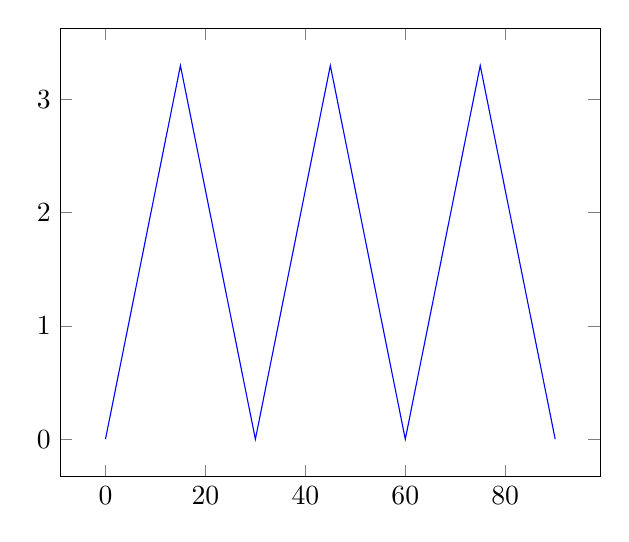
\begin{tikzpicture}
      \begin{axis}
        \addplot[color=blue] coordinates{(0, 0)(15, 3.3)(30, 0)(45, 3.3)(60, 0)(75, 3.3)(90, 0)};
      \end{axis}
    \end{tikzpicture}
    \label{Concept:Plot:zigzag}
  }
  % ramp
  \subfloat[][Rampenfunktion]{
    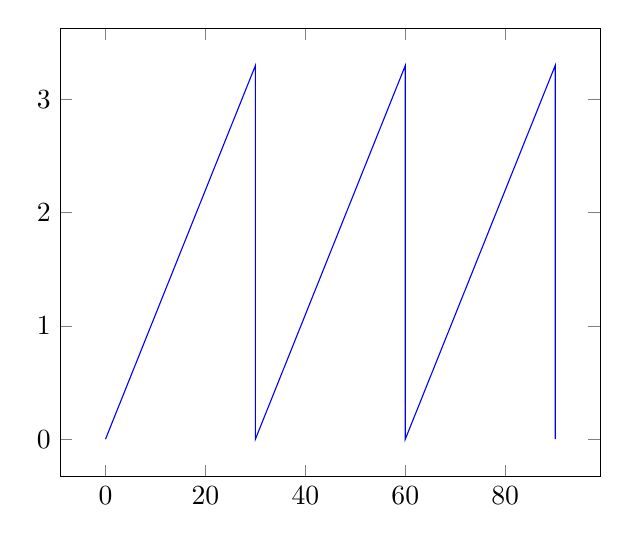
\begin{tikzpicture}
      \begin{axis}
        \addplot[color=blue, domain=0:90]  coordinates{(0, 0)(30, 3.3)(30, 0)(60, 3.3)(60, 0)(90, 3.3)(90, 0)};
      \end{axis}
    \end{tikzpicture}
    \label{Concept:Plot:ramp}
  }
  \caption{Funktionen} \label{Concept:Plot}
\end{figure}

\subsection{Konfiguration}
Der Funktionsgenerator muss, um 


\section{Aufbau}
Der Funktionsgenerator ist aus verschiedenen Einzelkomponenten zusammengesetzt.
Ihre Verschaltung im Generator ist in \cref{Concept:FuncGenDia} zu sehen.
Hier kann man gut erkennen, dass die verschiedenen Funktionen parallel arbeiten und von der Konfigurationsschnittstelle mit den Signalen \bitvect{cyc\_ticks}, \bitvect{high}, \bitvect{low}, \bitvect{thresh} und \bitvect{direction} gesteuert werden.
Das Signal \bitvect{waveform} steuert den Multiplexer, der die Ausgabesignale \bitvect{y\_out} an den DAC-Wandler weitergibt.
Dieser erzeugt daraus wiederum ein analoges Signal, dass dann am Ausgang anliegt.

\begin{figure}[h]
  \includegraphics[width=\textwidth]{function_generator}
  \caption{Diagramm des Funktionsgenerators, zusammengesetzt aus seinen Einzelkomponenten. Aus Gründen der Übersichtlichkeit sind die \bit{CLK} Signale und \lowactive{CE} Signale nicht angeschlossen dargestellt. Alle \bit{CLK} Signale sind an den Systemtakt angeschlossen und alle \lowactive{CE} Signale liegen auf Masse.}  \label{Concept:FuncGenDia}
\end{figure}

